Лектор Виктория Юрьевна Барсукова

ДУ - дефференциальное уравнение.

OДУ - обыкновенное дефференциальное уравнение.

$y(x)$ - ОДУ

$y(t_0, t_1, \ldots, t_n)$ - частные ДУ

Задачи решаемые ОДУ

1) Найти закон движение тела с заданной постоянной скоростью $\upsilon$
$$
s' (t) = \upsilon
$$
$$
s (t) = \upsilon t + C
$$

2) Найти закон движение тела при постоянном ускорения
$$
s'' (t) = a
$$
$$
s'(t) = at + C_1
$$
$$
s(t) = \frac{at^2}{2} + C_1 t + C_2
$$
или если известна начальная скорость и положение, то
$$
s(t) = \frac{at^2}{2} + \upsilon_0 t + v_0
$$

3) Задача о расходе радиактивного вещества. Известно что скорость распада радия
прямопрапарциональны его количества $m(t)$. Опредилить закон изменения $m(t)$

$$
m'(t) = k m(t)
$$
$$
m(t) = c e^{kt}
$$
$$
m(t_0) = c e^{kt_0} = m_0 ~~~ c = m_0 e^{-kt_0}
$$
$$
m(t) = m_0e^{k(t-t_0)}
$$

\begin{define}
  ОДУ называется уравнение содержащее неизвестную функцию одной переменной и ее
  производные или дифференциалы т.е. уравнение вида

  $F(x, y(x), y'(x), \ldots, y^{(m)} (x)) = 0$ или
  $F(x, y(x), dx, dy, d^2 x, d^2 y, \ldots d^n x, d^n y) = 0$

  $$
  y'(x) = \frac{dy}{dx}
  $$
\end{define}
Примеры:

1) $y'(x) = 2 y(x) + x$ может быть записана так $y' = 2y + x$ $y(x)$ - искомая
функция

2) $x'''(t) = x'(t)$

3)

$ydx + xdy = 0 ~~ / dx ~ y + xy' = 0$

$ydx + xdy = 0 ~~ / dy ~ yx' + x = 0$

\begin{define}[порядка уравнения]
  Порядком уравнения называется максимальный порядок производной или
  дифференциала входящего в уравнение.
\end{define}

\begin{define}[решения ДУ]
  Решение ДУ называется функция определенная на $<a,b>$ дифференциируема столько
  раз каков порядок уравнения и которая при подстановке в уравнение обращает его
  в тождество.
\end{define}
Пример:

$x''(t) + xt = 0$

$x''(t) = -x(t)$

$\varphi(t) = C_1 \cos t$

$\psi(t) = C_2 \sin t$

$x(t) = C_1 \cos t + C_2 \sin t$

\begin{title}
  Уравнения первого порядка
\end{title}

$F(x, y(x), y'(x)) = 0$ или $F(x, y(x), dy, dx) = 0$

$y'(x) = f(x, y(x))$ - уравнение разрешено относительно производной. Тоже что
$\frac{y(x)}{dx} = f(x, y(x))$

$f(x, y)$ - заданая функция с двумя независимыми переменными. Будем считать что
эта функция определена и непрерывна в некоторой односвязной области $D$.

\begin{center}
  Вопросы решаемые ДУ
\end{center}

1) существует ли решение ДУ

2) сколько решений существует ДУ

3) методы нахождения решения ДУ

4) устойчивость к изменениям ДУ

\begin{define}
  Пусть функция $y = \varphi (x)$ определена на $<a,b>$. $\varphi (x)$
  называется решением уравнения $y'(x) = f(x, y(x))$ если

  1) $\varphi (x)$ диференциируема на $<a,b>$

  2) $\forall x \in <a,b> ~~~ (x, \varphi(x)) \in D$

  3) $\frac{d\varphi (x)}{dx} \equiv f(x, \varphi(x)) ~~ \forall x \in <a,b>$
\end{define}

\begin{define}
  Задачей Коши для уравнения $y'(x) = f(x, y(x))$ называется следущая задача
  найти такое решение уравнение уравнения которое при заданом $x$ принимает
  заданное значение $y_0$
\end{define}
Пример:
$$
\left\{
\begin{array}{l}
  y'(x) = f(x, y(x)) \\
  y(x_0) = y_0
\end{array}
\right.
$$

  Общим решением уравнения $y'(x) = f(x, y(x))$ называется функция $y = y(x,c)$
такая что при $\forall C$ функция является решением уравнения и $\forall$
решение уравнения входит в это семейство при некоторых $C$.

  Решение при конкретном $C$ называется частным решением.

$xdy + ydx = 0$ тоже что и $d(x,y) = 0$

\begin{title}[\Large]
  Гометрический смысл уравнения первого порядка
\end{title}

$y' = f(x,y) ~~~ y'(x) = \tg \alpha$

$f(x, y) = A$ - изоклин

Пример:

$y' = y - x ~~~ y - x = A $

$A = 0 ~~~ y = x$ если $y > x$ то $y' > 0$ тогда $y$ возрастает

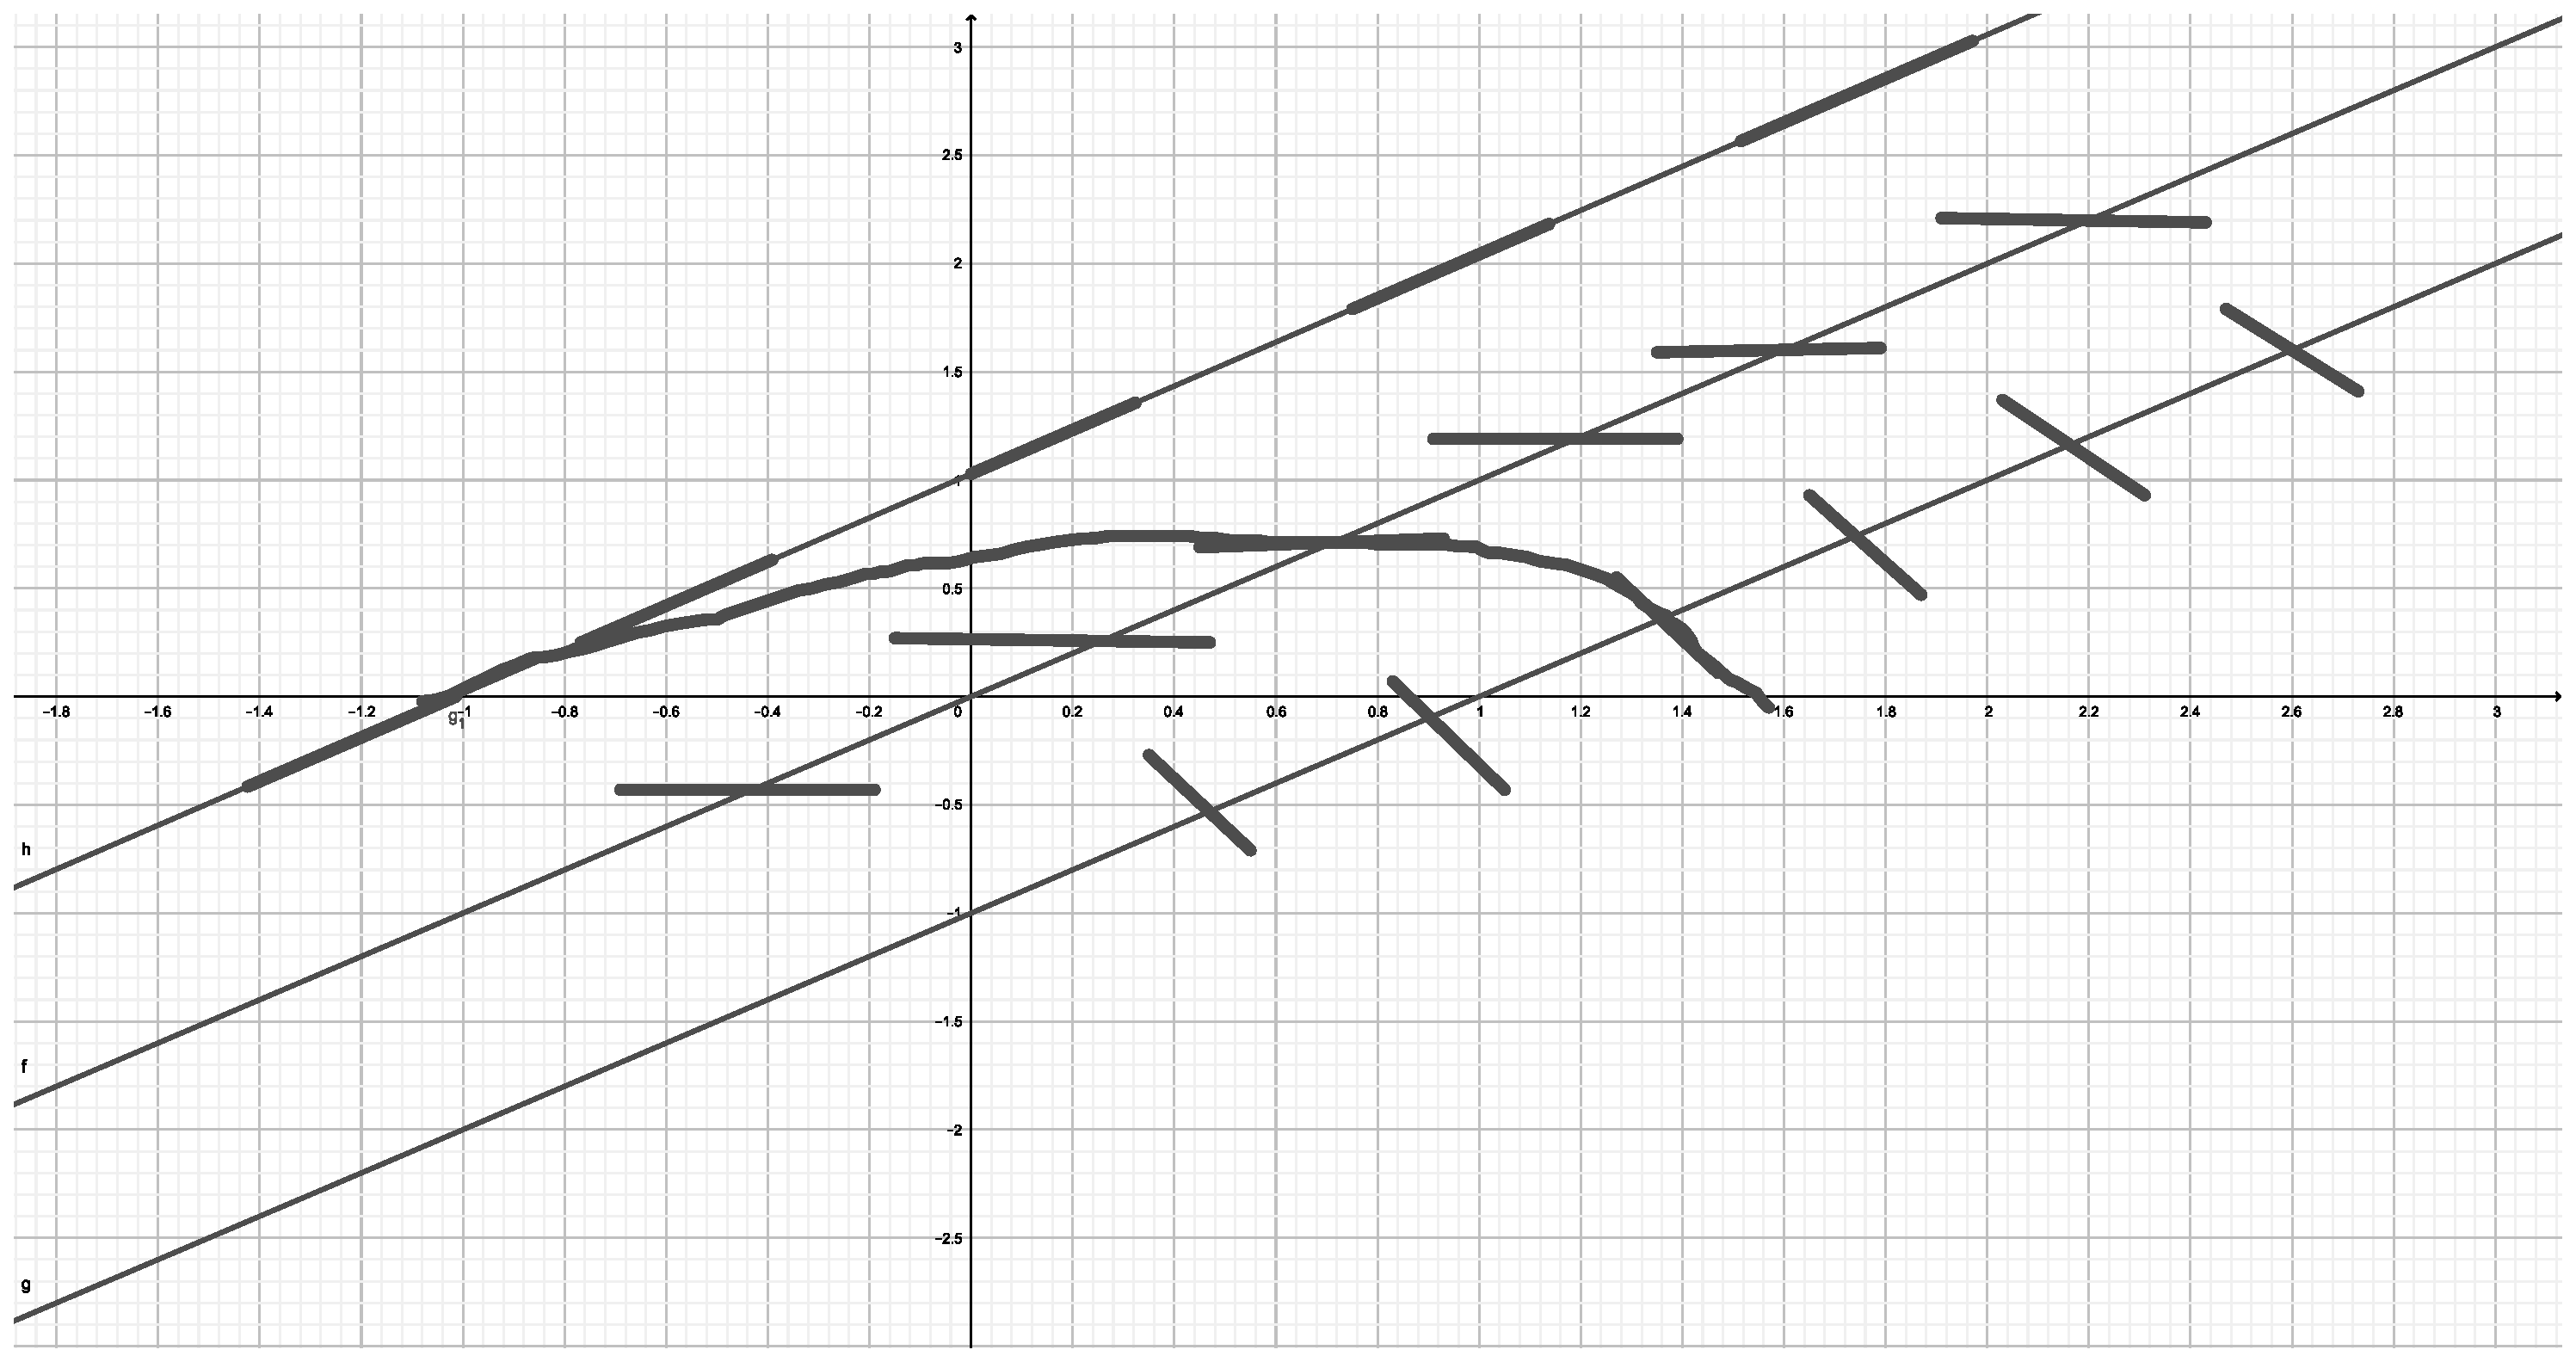
\includegraphics[width = 5cm]{geomFirstEqus}

\begin{title}
  Интегральные типы уравнений
\end{title}

$y'(x) = f(x, y(x))$
$$
y'(x) = f(x) ~~~ y(x) = \int f(x)dx
$$
$$
y'(x) = x^2 ~~~ y(x) =\frac{x^3}{3} + C
$$
$$
\left( \int_a^x f(x) dt \right)' = f(x) ~~~ \int f(x)dx = \int_a^x f(t)dt + C
$$
$$
y(x) = \int_{x_0}^x f(t)dt + C ~ \text{- общее решение}
$$

Решить задачу Коши
$$
y(x) = \int_{x_0}f(t)dt + y_0
$$